\lab{Computer Caches}{Caches}
\objective{Caches play an important role in computational performance.  Computers store memory in various caches, each with its advantages and drawbacks.  We discuss the three main levels of caches. Cache lines and cache sizes are discussed, along with CPU starving.}

The real computational bottleneck of computers lies in the memory system, not the processor.
In the early days of computing, memory speed and CPU speed were evenly matched.
The CPU accessed data directly from RAM without creating bottlenecks.
Now, the CPU spends a large amount of time waiting for data to process.
RAM simply isn't fast enough to keep up.  With CPUs crunching numbers at faster and faster rates, higher performance memory needed to be placed between a relatively slow RAM and the CPU to cache data.
This topic can very quickly become extremely technical.
The aim of the exercises in this lab are to provide a general knowledge of caching and its impact on performance.


\section*{Caching}
% TODO: add pictures of a library room with elements of this story.
A small story may help explain why we care about caching.
Imagine that you are working on an academic thesis.
Your thesis covers a very complicated topic and you need to reference a great number of papers and other resources.
It's late at night and your are alone.
You select a smallish desk that you will use for writing.
You decide to start by looking up a long list of books and their call numbers.  Bringing back as many books as you can carry, you commence writing.
Not surprisingly, you quickly discover that your desk simply is not big enough to hold all the books that you brought back.
You spot an unused library cart standing by a nearby wall.
Bringing the cart over to your desk you use it to store books that are not currently being used.
The cart also is useful for queuing books that will you will soon use.
However, searching the cart for a particular book soon becomes tiresome.
Not only do you have to find the book, but you have to find the correct page number.
You see a medium-sized table not far from your desk.
You decide to move the table adjacent to your desk so you can place open books on the desk.
As you work through the night and early hours of the morning, you establish a very efficient system.
Every hour or so, you collect books from off the shelves using the library cart, returning unused books back to the shelves.
Books that you need soon are placed on the large table, and books needed immediately are placed directly on your desk.
You notice that your most used books stay on your desk, while useful, frequently referenced books stay open on the large table.
As the first rays of sunlight shine through the east library window, you place the last finishing touches on your thesis.
What you have mimicked to some degree is the caching system of modern computers.

Caches were introduced to keep often-used memory accessible very quickly.  High speed memory is very expensive; there are economical constraints on how much cache is available in a CPU.
Another constraint is efficiency.  The faster the memory cache, the smaller it must be.
A final constraint is size.  The fastest levels of cache need to physically be close to the processing units of a CPU.
Today, there are several levels of cache located on the same chip as the CPU.

Caches are effective in two main scenarios: temporal locality and spatial locality.
Temporal locality describes the situation where we reuse specific parts of memory over and over again.
In our story, these would be books that we referred to many times.
These often-used memory locations are cached to make them more quickly accessible.
Spatial locality describes the situation where we access memory locations that are close together.
In our story, these books are physically located close to each other on the shelves.
We can cache a particular memory address and all the addresses around it as well.
Today's caches can also try to predict what data will be needed next and pre-fetch it from slower levels of memory.
If we use algorithms that can take advantage of these two data usage patterns, caching will provide a tremendous speed boost.
However, if we are not intelligent in our choice of algorithm, we will be forcing the CPU to sit idle as it waits for data to be fetched from main memory.
The optimal strategy for an efficient algorithm is to fetch sequential blocks of data and reuse them as much as possible before requesting more data from main memory.
For the last few decades, the bottleneck in performance has been memory speed, not processor speed.

\section*{Cache Lines}
The cache is made up of \emph{cache lines}.
Cache lines contain blocks of bytes that have been fetched from main memory.
Accessing other bytes within the same cache line has close to no overhead.
When a requested byte is already in cache, it is called a \emph{cache hit}.
We can measure the cache line size by reading values from a large array of 32 bit (4 byte) integers.
For example, if we have 64-byte cache lines, then reading one integer from the array will also pull in the next fifteen, because $4 \mbox{~bytes} * 16 \mbox{~integers} = 64 \mbox{~bytes}$.
So if we read in every integer, or every other integer, or even every sixteenth integer, we will have to load the entire array into the cache, one line at a time.
With step sizes larger than 16, however, we are not fetching the entire array into cache because there is a gap between each integer read and the end of the previously fetched cache line.
\begin{figure}[h]
\centering
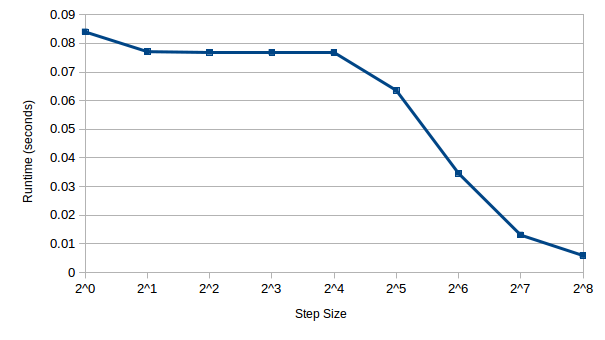
\includegraphics[width=\textwidth]{cache_line.png}
\caption{Determining cache line size by looping through a 128MB array with different step sizes. Note the dropoff at 16 corresponding the the cache line size.}
\label{fig:linesize}
\end{figure}

\begin{problem}

Find the cache line size for your machine.  To do this, create an array of size $2^{18}$. You will need to make a function that accepts no arguments which reassigns a new value for every $i^{th}$ element of the array.   Use powers of two for your values of $i$.  Using the mean value obtained by the \li{timeit.repeat} function, assign a timing for each value of $i$.  The main argument for this function will be the name of the function you created.  As additional keyword arguments, use \li{repeat=10} and \li{number=1000}.  Plot your results on a graph like Figure \ref{fig:linesize}, using a line with square markers.  Your results should be comparable to the figure.

\label{prob:cacheline}
\end{problem}

\section*{Cache Size}
% TODO: insert graphics that illustrate the memory hierarchy
Various levels of caches were inserted between main memory and the CPU.
As cache sizes grow, their access times slow down.
Level 1 (L1) cache was wired directly into the processor.  Level 2 (L2) cache is also wired directly into processor.
Many multi-core processors these days have a third (L3) cache in addition to L1 and L2 caches.
L1 cache is the smallest at around 32 kilobytes, with the fastest access times of around 1 nanosecond.
In our story, this was represented by the writing desk.
L2 cache comes in at about 3 nanoseconds.  L3, the largest but slowest of the caches, clocks in at about 10 to 20 nanoseconds.
The library table represented L2 and L3 caches.
Main memory finally takes about 100 nanoseconds to access.  While 100 nanoseconds is really quick in our perception of time, it is a really long time in the processor's measurement of time.
The library cart represented main memory.
A \emph{clock cycle} is the fundamental unit of time for a processor.
Accessing data from L1 cache takes about 4 clock cycles on modern processors.  Fetching data from L2 cache takes about 10 clock cycles, and from L3 about 75 clock cycles.
Fetching data from RAM takes several hundred clock cycles.
Each cache stores a subset of the cache above it.  L2 contains a copy of all of the data in L1, L3 has a copy of all of the data in L2 and so on.
Requesting data from mass storage like a hard drive or optical disc takes millions of clock cycles.  In processor time, this is basically an eternity.
If a clock cycle is equated to one second, fetching data from the hard drive would take about 1 year.
This is why caching is important.  Operating systems generally use part of RAM as a cache for the hard drive.

We can measure the drops in performance that occur when we overflow the cache (Figure \ref{fig:cachesizes}).
We performed measurements on an Intel i7-2640M processor.  The cache line size is 64 bytes (the size of 16 32-bit integers).
\begin{figure}[h]
\centering
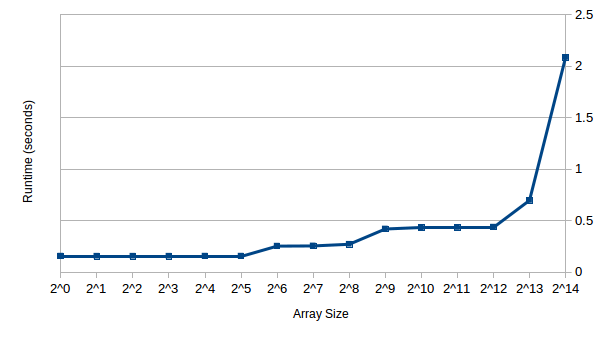
\includegraphics[width=\textwidth]{cache_size.png}
\caption{The increases in runtime occur at 32KB, 256KB and 4MB, which correspond to the sizes of L1, L2, and L3 caches.}
\label{fig:cachesizes}
\end{figure}

\begin{problem}
Measure the size of your L1 and L2 caches using the cache line value obtained in
Problem \ref{prob:cacheline}.
To compile you the included C program, you will need a C compiler.
We recommend gcc with the flags \texttt{-O3 -mtune=native}.
The C program expects three arguments: first, the candidate array size, second, the cache line size, and third, the number of loops to run during testing.
The program will print out how many seconds on average one loop took to execute in seconds.
Plot the results of your measurements.
\end{problem}

\section*{Solutions to CPU Starving}
\emph{CPU starvation} refers to the condition of having to wait a relatively long time for data to compute.
The way to solve the CPU starvation problem is to be aware of how your data is laid out in memory.
NumPy has support for two main types of memory layouts for arrays:
% TODO: add illustration of row major vs, column major format for arrays.
\begin{description}
\item[Row-major:] Arrays are stored by rows in continuous memory.
Languages such as C and Python use row-major indexing.  NumPy arrays by default use this indexing convention.
Slicing down columns is slow.  In NumPy, row-major arrays are identified as \emph{C contiguous} (\li{order='C'}).
\item[Column-major:] Arrays are stored by columns in contiguous memory.
Languages like FORTRAN, MATLAB, and R use column-major indexing.  Slicing across rows is slow.
In NumPy, column-major arrays are identified as \emph{FORTRAN contiguous} (\li{order='F'}).
\end{description}
Paying attention to how your arrays are indexed will be beneficial to the performance of your algorithms.
Some algorithms work better with a particular type of indexing.

While NumPy is very fast for most purposes, it has a tendency to create many temporary arrays as it evaluates results.
The code below will result in the creation of many different arrays, each the size of \li{x}!
Calculating $y$ takes about one second on a typical machine.
\begin{lstlisting}
x = np.linspace(-1, 1, 10*1024*1024)
y = 1.25*x**3 - .33*x**2 + .75*x + 1.2
\end{lstlisting}
We can reduce the runtime by using a little bit of algebra.
Factoring the expression results results in a much easier expression for the computer to evaluate.
Calculating the equivalent expression takes $.146$ seconds!
\begin{lstlisting}
y = ((1.25*x - .33)*x + .75)*x + 1.2
\end{lstlisting}
A tremendous speed up for not a whole lot of work.

Numexpr, a library for Python, is designed to utilize the CPU cache as well as avoid unnecessary temporary arrays.
It evaluates the following expression allocating only a single array and operating on $x$ in blocks that fit into the CPU cache.
It calculates the entire expression for that particular block, then saves the result.
One a typical machine, numexpr can execute the unfactored expression in $.0387$ seconds and the factored expression in $.0349$ seconds.
\begin{lstlisting}
import numexpr as ne
yne = ne.evaluate('1.25*x**3 - .33*x**2 + .75*x + 1.2')
\end{lstlisting}
Using Numexpr instead of NumPy can speed up simple vector computations significantly.
These large gains in performance are primarily for large arrays.
Numexpr will operate on these large arrays in blocks that fit into the CPU cache.
Numexpr is also designed to easily take advantage of multiple cores by default, a feature that NumPy lacks.
The above evaluations using Numexpr were done using 4 threads.
Please refer to the Numexpr Users Guide (\url{https://code.google.com/p/numexpr/wiki/UsersGuide}) for information on what operations are supported by Numexpr.

Many scientific libraries have been optimized to utilize the CPU cache.
Libraries like LAPACK and BLAS have been tuned by many experts to efficiently use memory.
Other packages, like ATLAS (an alternative BLAS implementation), can automatically tune their algorithms to optimize performance on a particular platform.
